
\documentclass{article}

\usepackage[activate={true,nocompatibility},final,tracking=true,kerning=true,spacing=true,factor=1100,stretch=10,shrink=10]{microtype}
% activate={true,nocompatibility} - activate protrusion and expansion
% final - enable microtype; use "draft" to disable
% tracking=true, kerning=true, spacing=true - activate these techniques
% factor=1100 - add 10% to the protrusion amount (default is 1000)
% stretch=10, shrink=10 - reduce stretchability/shrinkability (default is 20/20)

\usepackage[utf8]{inputenc}
\usepackage{amssymb}
\usepackage{amsmath}
\usepackage{mathtools}
\usepackage{svg}
\usepackage{graphicx}
\usepackage[superscript, biblabel, nomove]{cite}
\usepackage[hidelinks]{hyperref}
\usepackage{cleveref}
\usepackage{tikz}
\usepackage{pgfplots}
\usepackage{datetime}
\usepackage{color}

\pgfplotsset{width=7cm,compat=1.9}

% use "\head" to define table heading formatting
\newcommand{\head}[1]{\textnormal{\textbf{#1}}}

% Use § for sections
\crefformat{section}{\S#2#1#3}
\crefformat{subsection}{\S#2#1#3}
\crefformat{subsubsection}{\S#2#1#3}

\usepackage{appendix}

% == Remove or comment these out for release
%\usepackage{todonotes}
%\usepackage{draftwatermark}
%\SetWatermarkText{DRAFT}
%\SetWatermarkScale{3}
% ==

\usepackage[utf8]{inputenc}
\usepackage[english]{babel}
\usepackage{amsthm}

% Make itemize bullets slightly smaller
\renewcommand\labelitemi{{\boldmath$\cdot$}}

\newtheorem{theorem}{Theorem}
\theoremstyle{definition}
\newtheorem{definition}{Definition}[section]

\newtheorem{thm}{The`orem}[section] % the main one
\newtheorem{lemma}[thm]{Lemma}

\theoremstyle{plain} % just in case the style had changed
\newcommand{\thistheoremname}{}
\newtheorem{genericthm}[thm]{\thistheoremname}
\newenvironment{namedthm}[1]
  {\renewcommand{\thistheoremname}{#1}%
   \begin{genericthm}}
  {\end{genericthm}}


\begin{document}

% Macros
% nil

\title{Enosi Green Paper\\ v0.3}
\author{Samuel Brooks, Matthew Hale, Steve Hoy}
\date{}

\maketitle

\hfill

\begin{abstract}
\noindent Modern energy markets are structurally inefficient, resulting in higher-than-neccessary electricity prices and frustration of investment into appropriate renewable infrastructure.
Grid 2.0 technologies, including cheaper solar power, can optimise the generation and distribution architecture of aging energy networks and slash cost from the energy stack.
Critically, electricity companies in commercial competition with one another within a given energy market naturally segment the customer base, resulting in structurally sub-optimal risk management for the purchase and provision of electricity. By using distributed ledger technology, the Enosi system splits this business model into two, thereby creating a competitive market for load profiles and optimising credit risk, resulting in lower electricity prices for end consumers.
\end{abstract}
\vspace{20mm}
\begin{center}
  %\color{gray}
  \small{\textit{\today}}
\end{center}

% \todo[inline]{Incorporate white paper criticisms.}

\pagebreak

\tableofcontents

% == Remove or comment out this section for release
% \pagebreak
% \section{TODO}
% \listoftodos{}
% ==

\pagebreak

%\input{tex/introduction}
%\input{tex/design_considerations}
%\input{tex/system_description}



% \appendix
% \appendixpage
% \addappheadtotoc
%\input{tex/alternative_approaches}
%\input{tex/system_variables}

%\bibliography{tex/citations}
%\bibliographystyle{plain}


\section{Introduction}

Globally, it is now clear that a number of issues have resulted from a centralised power generation architecture, including a power-inefficient transmission system, the stimulation of the use of fossil fuels in order to extend the life of existing assets, and regulation which supports incumbency and stymies innovation. Even though Australia is one of the most deregulated energy markets in the world, it structurally inhibits local (distributed) generation and consumption. \\

\noindent Enosi seeks to provide the means for small and startup energy businesses and not-for-profit entities to compete in established markets. Providing such an equal opportunity fosters competition with incumbent players, allowing more competitive and more relevant services to be offered to energy consumers, such as the facility for localised peer-to-peer energy trading, control over the provenance of their electricity, and transparency of cost. \\

\noindent The key enabler for this shift is the ability for all actors in a retail energy market to access a shared understanding of (i) energy usage data and (ii) pricing and settlement logic that acts over that data. Distributed ledger technology enables us to build such shared data and logic systems, including standardised software and business process workflows. Indeed, cryptographically-secure methods of sharing both information and logic are the only way to orchestrate the necessary cooperation to achieve the economies of scale necessary to provide localised services and price-efficient community energy. By taking full advantage of distributed ledger technology, as well as “Grid 2.0” technologies such as smart meters, we can create very efficient networks of interconnected retailers, Neo-retailers and end-consumers who both cooperate and compete with one another.\\

\noindent Enosi is developing a distributed ledger software platform to provide the tools and network effect to enable small and community-based actors to disrupt established energy market players. It is a not-for-profit foundation developing this platform as free software but with an associated a Network-as-a-Token model, and will be initially funded as an ICO. While the software will be made open source, the token is required to access individual energy networks (geographical markets).\\

\noindent "We are here to change the electricity industry, because the incumbents won’t."\\
- Stefan Jarnson, Enosi Project




\pagebreak
\section{Solution Description}

\subsection{Problem Space}

Currently, there exists two key structural inefficiencies in modern energy markets: fragmented risk management, and misaligned investment incentives. We explore these in turn.

\subsubsection{Inefficient buying risk management}

The first is the segregation of loads due to customer segmentation within a market; most customers within an energy market are contracted to a small number of large energy companies to provide their electricity. These companies manage their own buying risk with the wholesale electricity market (power generation companies sell into this wholesale market). Modern electricity regulation in most jurisdictions globally require continuity of service for end-consumers, and this means that protections exist for generation companies against the interposing energy retailer mismanaging its balance sheet and being unable to pay the generators for the electricity it is required to buy and supply to its customers. This protection takes the form of a credit or bond held on trust with the local regulator in the event that the retailer cannot pay its bill to the wholesale market. However even within this context, energy retailers still seek to make a profit, and this can only be achieved by improving the efficiency of their risk management in buying power from the wholesale market and selling it to end consumers. Where this done improperly, and in the case where wholesale prices skyrocket such as in an adverse weather event, it can lead to the prompt failure of the business.\\

\noindent Because the market is segregated between these energy retailers who are in competition, an optimal risk management strategy is never able to be achieved; the most efficient scenario is one where all customer load profiles, both commercial and residential, are aggregated to produce a ‘flat’ a demand as possible, making the prediction of what electricity is necessary to purchase as accurate as possible. A completely predictable load profile is one which can be easily satisfied, and the greater the number of customers within a market smooths out this load profile making it more predictable.

\subsubsection{Grid management incentives}

In addition, incumbent companies in some jurisdictions are not appropriately incentivised to maintain an inefficient grid. Reduction of capital expenditure for the utility.

Nelson bay example.

<steve to add info on this>.

\subsection{Solution Space}

The key to unlocking value in these energy markets is to reconfigure the market with a different set of actors who can interact in a fundamentally more efficient way. Specifically, we propose decomposing the traditional energy retailer into two distinct parts: a wholesale Licensed Supplier, and a Neo-retailer.\\

\noindent \textbf{Licensed Supplier}: a company or not-for-profit entity who buys electricity from the wholesale market and sells it into the retail market, typically via a Neo-retailer. Licensed Suppliers are required to abide by existing prudential regulations, including holding capital to protect creditors (electricity generation businesses) against a failure of their credit risk operations.\\

\noindent \textbf{Neo-retailer}: a company or not-for-profit entity who specialises in providing customer-facing services, including customer acquisition, metering, billing, and ancillary services such as peer-to-peer energy functions. Neo-retailers do not require an electricity market license, and so may be operated by anyone, including not-for profit community groups, or tangentially related business (such as electric vehicle manufacturers) who can market more specific value propositions to their customers.\\

\begin{figure}
\begin{center}
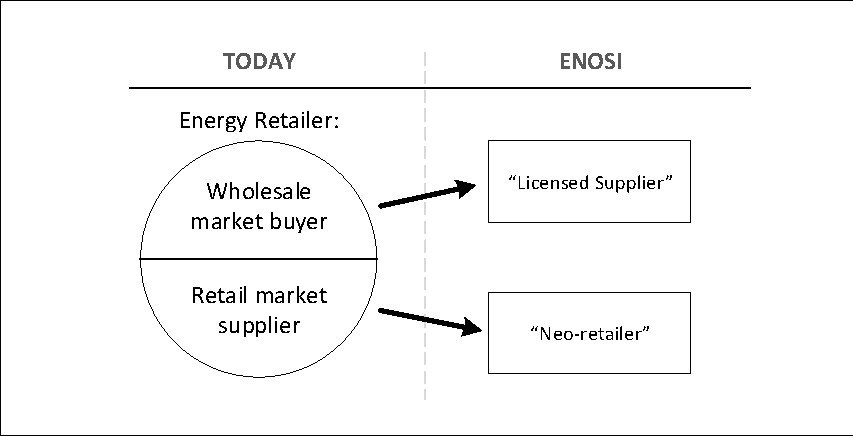
\includegraphics[width=250pt]{/home/samuel/dev/block8/green-paper/enosi-retailer-split.pdf}\\
\caption{Splitting of the traditional retail energy business.}
\end{center}
\end{figure}


\noindent The effect of this will be to:

\begin{itemize}
\item{Create a single marketplace for Neo-retailers to acquire customers, and for Neo-retailers in turn to publically advertise and on-sell their unique customer load profile to Licensed Suppliers. This enables Licensed Suppliers to compliment their sell profile in order to optimise their buying profile, and in turn offer more competitive pricing to the Neo-retailer.}
\item{Reduce the cost of customer management functions by supporting not-for-profit entities to act as Neo-retailers. Such entities will be structurally more competitive than traditional for-profit service companies, resulting in cheaper electricity prices for end-customers.}
\item{Create a more diverse set of Neo-retailers more able to satisfy the needs of customer subgroups.}
\item{Accelerate the use of smart metering as Neo-retailers can form around this technology to offer even cheaper and more efficient retailing services by removing the need for manual meter-reading.}
\item{Accelerate the use of distributed generation (e.g. rooftop solar) as it becomes easier for actors to enter the market and offer peer-to-peer services.}
\end{itemize} 

\noindent Creating such a network is achievable by using distributed ledger technology to efficiently share metering and customer data as well as adhere to a common standard for the energy retailing stack. Having all market actors running common software to standardise energy data (e.g. metering) and logic (e.g. billing) means that interoperation between market players becomes possible; it would be impractical to integrate together every disparate system that currently exists, or create a separate for-profit company dedicated to interfacing between them all. It is only via the creation of a not-for-profit foundation, run by individuals who are incentivised to improve the value of the network, does such a singular network become possible. \\

\noindent Enosi is therefore tasked with building the software that enables these interactions, thereby reducing the cost stack for Neo-retailers and enabling Licensed Suppliers to more effectively hedge their wholesale risk by accessing the aggregated load profiles of consumers. \\

\begin{figure}
\begin{center}
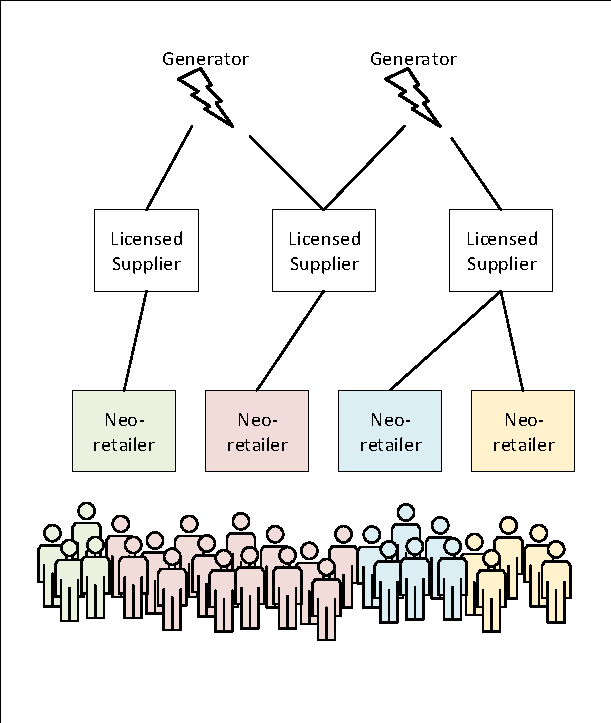
\includegraphics[width=200pt]{/home/samuel/dev/block8/green-paper/enosi-stack.pdf}
\caption{Separation of licensed and retail entities in the energy stack.}
\end{center}
\end{figure}

\noindent As the network grows and matures over time, it will create second-order incentives for Licensed Suppliers to cooperate (and ultimately aggregate into super-operators) in order to continue to take advantage of sell-side aggregation of load profiles. This network will naturally dissolve a fragmented market through an increasing number of cooperative agreements. Because Neo-retailers are in custody of their own data and logic (including a customer identity), and that within the market Neo-retailers are able to easily switch between their electricity supplier, this aggregation cannot cause anti-competitive monopolies.

\begin{figure}
\begin{center}
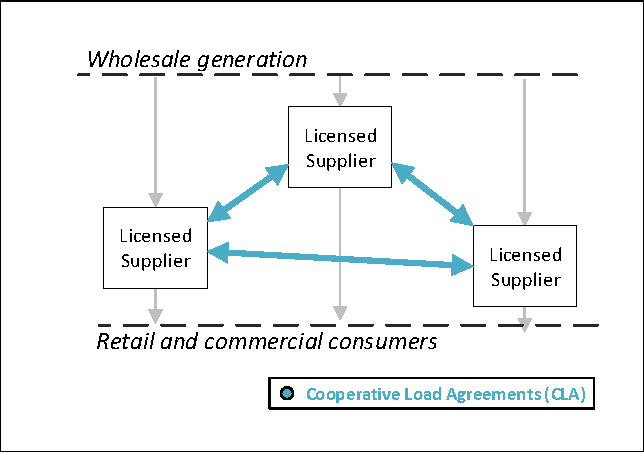
\includegraphics[width=300pt]{/home/samuel/dev/block8/green-paper/enosi-cla.pdf}
\caption{Financial agreements between wholesale energy traders.}	
\end{center}
\end{figure}

\subsection{End state}

The ultimate arrangement of the network within a given market will see maximal connectivity between Licensed Suppliers and Neo-retailers who follow their incentives. Once this process reaches its equilibrium, the end-state of the network will effectively become a Distributed Autonomous Organisation (DAO) functioning as a wholesale market player that is owned and governed by Neo-retailers and community members. In this end state, the regulatory environment will be ready to be reformed to bring wholesale buying into the ecosystem as well. In this scenario, the various aggregated wholesale buying entities will be replaced by a single DAO, per wholesale jurisdiction, that would handle all the wholesale market interactions on behalf of the Neo-retailers. \\

\noindent At this point in time, the way energy is procured and distributed to Neo-retailers and eventually end-consumers is run entirely for the community via market Enosi DAOs (EDAO). The Enosi project is breaking apart the existing inefficient retailer model and rebuilding it with the community at the centre.\\

\noindent The cryptoeconomic incentive scheme supporting this network effect, including the use of the \textbf{Joul}, is described in later sections.

\subsubsection{Actor definitions}

A summary of the various actors and their role in the ecosystem is given below:\\


\begin{tabular}{|l|l|}
 \hline 	
 \head{Actor} & \head{Motivations and Use of Joul}\\
 \hline 
 \hline
 
 \textbf{Consumer}:				& \\
 \hline 
 Consumer/prosumer of 	 		& Wants cheaper electricity and the ability to	\\
 energy who is a member  		& trade directly with peers. Procures Jouls to	\\
 of a Neo-retailer or EDAO.		& directly participate in the network within a	\\
  								& DAO, or joins as a member of a Neo-retailer	\\
 								& who procures Joul on their behalf. 			\\
 \hline

 \textbf{Neo-retailer}:			& \\
 \hline
 Entity providing a consumer	& Wants to facilitate Grid 2.0 energy services	\\
 interface to the wholesale 	& to customers with their unique value 			\\
 market, including billing 		& proposition. Stakes Jouls in order to access 	\\
 and exception management 		& the Enosi network.							\\
 functions. 					& \\ 
 \hline 
 
 \textbf{Licenced Supplier}:	& \\ 
 \hline
 Financially responsible 		& Wants to access additional customers to 		\\
 market participant (FRMP), 	& obtain a better risk position on the			\\
 interacting with the 			& wholesale market. Stakes Jouls in order to 	\\
 wholesale energy market and 	& access the Enosi network.						\\
 supplier to the retail market.	& \\
 \hline 
 
 \textbf{Application Provider}:	& \\
 \hline 
 Third party offering services	& Wants to provide goods and services to 		\\
 to actors on the Enosi 		& actors on the Enosi network. Currently no 	\\
 network, such as a metering	& need to acquire Jouls to pariticpate.			\\
 data provider.					& \\
 \hline
 
 \textbf{Enosi Foundation}:		& \\
 \hline 
 Facilitator of the ecosystem.	& Wants to build and maintain the 				\\
 Manages the staking function	& infrastructure required to support the 		\\
 for the network.				& Enosi network. Recieves a fee in Jouls each	\\
 								& time they are traded in the ecosystem.		\\
 \hline 

 \textbf{EDAO}:					& \\
 \hline 
 Enosi Decentralised 			& Acts only as programmed. Jouls sourced by		\\
 Autonomous Organisation.		& members are used to stake for the continued	\\
 Functions like a Neo-retailer	& participation in the network. \\
 without central governance. 	& \\
 centralised governance.		& \\
 \hline
\end{tabular}


\subsection{Trust Design}

In order to understand how to develop smart contracts between the defined actors, we must understand which of those actors are in a natural financial contention, that is, for which actor pairs do we need to write trust management programs into the Enosi permissioned distributed ledger system? \\

\noindent We consider the following trust relationships as they exist today and how they can be automated:

\begin{itemize}
\item{\textbf{Current}: Customers trust that billing is accurate and fair between them and their "Retailer" (Licensed Supplier). \\

\textbf{To be}: A permissioned distributed ledger is used to prove the calculation of the customer’s electricity bill.} \\

\item{\textbf{Current}: Customers trust that their Licensed Supplier will reliably supply them with energy from the wholesale market.  Generators trust that Retail License Holders will accurately/effectively settle the ‘overs and unders’ between the wholesale market and the downstream markets (Neos and communities) \\

\textbf{To be}: Customers and Neos trust that their Retailer will reliably supply them with energy from the wholesale market. Retail License Holders will accurately/effectively settle the ‘overs and unders’ between the wholesale market and the downstream markets (Neos and communities)?} \\

\item{\textbf{Current}: Customers trust that their data is kept secure and is accurately maintained. \\

\textbf{To be}: All system participants can verify the veracity of data. Customers have control over the accuracy and permission settings over their data. Data resides encrypted on a permissioned distributed ledger and customers provide permission for the storage of their data under this regime.} \\

\item{\textbf{Current}: All participants trust smart meters and meter data providers (MDPs) for metering information. \\

\textbf{To be}: No change to the current market, however Neo-retailers providing services to customers only with smart meters should result in cheaper pricing.}
\end{itemize}

\noindent Hence, we can define the following transactional relationships more formally from the base actor types: Licensed Supplier, Neo-retailer and Consumer:

\begin{itemize}

\item{ \textbf{Licensed Supplier - Licensed Supplier}:
In commercial competition. Do not wish to share any data, including metering data. However, smaller Licensed Suppliers may benefit from sharing anonymised metering data and jointly buying wholesale hedges to match this aggregated demand profile.}

\item{ \textbf{Licensed Supplier - Neo-retailer}:
Neo-retailer acts as a sales channel for a Licensed Supplier. Neo-retailer only provides minimum required information to the Licensed Supplier. Neo-retailer only links in with the Licensed Supplier in order to gain pseudo-access a retail energy licence. Licensed Supplier wishes to acquire customers through Neo-reatilers and may incentivise them to access to their retail energy licence via a marketplace on the Enosi platform.}

\item{ \textbf{Licensed Supplier - Consumer}:
Consumer wishes to reduce their costs, while the Licensed Supplier wishes to maximise profits. Consumer needs the Licensed Supplier to take away the wholesale risk.}

\item{ \textbf{Neo-retailer - Neo-retailer}:
May or may not be in commercial competition. Larger, more 'commercial' Neo-retailers may well be in commercial competition in a similar fashion as two Licensed Suppliers.}

\item{ \textbf{Neo-retailer - Consumer}:
In some scenarios, a consumer may wish to reduce their costs, while a Neo-retailer may wish to maximise profit. In others, consumers wish to contribute to the community, while Neo-retailers wish to facilitate consumer contributions to the community.}

\item{ \textbf{Consumer - Consumer}:
There may be concerns that other consumers are bad actors wanting to exploit their data if shared with others. However, some communities might have a higher level of inherent trust than others and will share data with permissions.}

\end{itemize}

\subsubsection{Other requirements}

Other key elements to the interoperation of these actors includes:

\begin{itemize}
\item{ Identity standards for all standard actor types (e.g. a fully-featured consumer identity that satisfies the requirements of Licensed Suppliers, Neo-retailers and other consumers).}
\item{ Interfaces for external actors, such as regulators, to interact with the system. }
\item{ Standarised software for basic operational tasks, such as an interface to the load profile market, customer onboarding, billing and settlement functions.}
\end{itemize}



\pagebreak
\section{Value Definition}

\subsection{Value networks}

Blockchains are good at representing value as they resolve the double-spend problem for both digital assets and digital representations of real-world assets. All value in any asset is fundamentally derived from a network of participants of mutual belief, but while “real-world assets” derive their value from existing markets and agreed utility established over time, “crypto-assets” do not benefit from the tenure of well-known markets established over time. They do however still derive value from a network of participants who collectively agree on the value that the token represents.

\subsection{Value definition}

For Enosi, we define the fundamental value of the Enosi platform to be the following:\\

\noindent For consumers and prosumers:

\begin{itemize}
\item{Minimised electricity prices due to cooperative load agreements.}
\item{The means to undertake peer-to-peer energy trading.}
\item{The ability to be in better control on where you buy your power from.}
\item{The ability to have  over control your metering data and visibility of your billing logic.}
\item{The ability to act as your own energy retailer, ("Neo-retailer"), and cooperate with others to form a decentralised autonomous organisation (DAO)}
\item{The ability to efficiently change electricity retailers.\\}
\end{itemize}

\noindent For Neo-retailers:

\begin{itemize}
\item{The ability to provide specialised retail services without requiring a retail energy licence.}
\item{A means to access a marketplace of energy retailers and energy consumers.
The ability to access energy retail business software, including billing and metering processes.\\}
\end{itemize}

\noindent For retail energy licence holders, “Licensed Suppliers”:

\begin{itemize}
\item{A means to access benefits of scale, including minimising wholesale buying risk.}
\item{A means to access a pool of new energy customers.\\}
\end{itemize}

\noindent For all:

\begin{itemize}
\item{Aggregated data useful for third party analytics.}
\item{Brand awareness of this particular platform.}
\item{An operating Foundation supporting the development of this particular ecosystem.}
\item{The means to influence a greener and more decentralised energy future by incentivising the use of smart meters and distributed generation.\\}
\end{itemize}

\noindent The Enosi ecosystem facilitates new and innovative models of community oriented energy supply and management by providing the means to share energy-related data and logic. In most jurisdictions, this also democratises access to energy retail licensing by enabling businesses specialising in wholesale risk management, without the need to manage consumers. Currently, community-based organisations cannot currently become energy retailers without first obtaining an energy retail license. Today, this is a prohibitively costly and cumbersome process. With the successful implementation of the Enosi ecosystem and the market efficiencies that are unlocked, this idea of a truly community-based energy retailer becomes possible.

\subsection{Value representation}

Now that we have defined the value of the Enosi network, we then define a set of fungible cryptographically-secure tokens which represent this value. We recognise the difficulty in representing all forms of value in tokenised form, including data and open source software; that which is given away for free, and able to be freely copied, simply cannot have its value captured in the same way that a software licence can capture value. Hence, in our value definition, we have not defined the software itself as part of the value represented by the token.\\

\noindent The token then is an access token. It is required to access the permissioned Enosi network and allow interoperation with other network participants. Network permissioning is enforced through the ‘staking’ of tokens within a smart contract on a public blockchain, such as Ethereum. Once the staking requirements of the smart contract have been satisfied, permission is provided for the owner of that stake to join the network. Permissioning is managed by network consensus (however in initial versions this will be managed by Enosi centrally).\\

\noindent Thus, a token representing the value of a network can be used to pay for access to that same network. Such a recursive scheme is a neat way of supporting the value of the network as its value is directly measurable in the open (and ideally, efficient) market price of the token.\\

\noindent An access token for purely open source software and completely public data is difficult to maintain, however with the requirement for private information, we can use an access token to pay for access to network benefits (such as aggregated data), even if the software used by the network participants is made open source. In addition, there may be some conveniences which are reserved for platform participants, such as cloud deployment scripts for a network node.

\subsection{Alternative Token Models}

There are a number of potential alternative token utility models that are commonly found in cryptocurrency and blockchain literature. We briefly discuss two of these:

\begin{itemize}
\item{Tokenised electricity (tokenisation of an asset)}
\item{Settlement}
\end{itemize}

\subsection{Tokenised electricity}

Currently, grid power is always netted and so electricity is never stored or owed. It is always bought and sold, and then settlement occurs at a later time. Thus, there is rarely the situation where electricity can be held for value appreciation. In addition, the asset is ephemeral (it is typically only generated once and consumed once), and is difficult to transfer to a market outside the one in which it is geographically located. Thus it is a poor candidate to be a tokenised asset.\\

\noindent Tokenisation of power may become more relevant in future versions of the Enosi platform, however this will likely be represented with a different token. See section 7 for more details on how tokenised power may work.

\subsection{Settlement}

There are several challenges with tokens whose primary utility within their ecosystem is settlement. For our purposes, these will be called medium of exchange tokens.\\

\noindent In medium of exchange token ecosystems, tokens may cycle through the system as a whole very quickly. For example, if the network grows to be significantly large, the transactional volume of the token will be high, but so will the token velocity, i.e. how quickly tokens move through the system end to end.\\

\noindent A high token velocity is problematic because there is no incentive to hold the token and incur price risk relative to fiat currencies (or other cryptocurrencies, for that matter). This is because in order to settle, one simply needs to buy the required quantity of tokens at settlement, thereby increasing sell pressure at all other times. Fundamentally, if there is no need for regular users to hold on to the token then the token’s price is only linked to speculation.\\

\noindent Contrastingly, if everyone holds the tokens and no one is using them within the ecosystem or trading them outside of it, transactional volume collapses as does the price of the token because there is no demand. There is clearly a need for a delicate balance between incentives to hold tokens, and incentives to use them. Thus, a finely tuned token velocity is required when designing token economy mechanics.\\

\noindent Perhaps most critically, the price-volatile tokens and cryptocurrencies are effectively useless as means of settlement when pricing of goods and services is in fiat. Solving the volatility of cryptocurrencies is non-trivial and lies outside the scope of the Enosi project. Hence, settlement is not a part of the primary utility of the Joul token, and the function of settlement in the ecosystem remains to be implemented via the use of a stablecoin, digital fiat, or regular payment rails.



\pagebreak
\section{Token Mechanics}

\noindent The objective of the programming of the token (the Joul) is to encourage network cohesion; that is, incentivise the defined market actors to continue to interoperate with each other in order to support the benefits that arise from the existence of the network.

\subsection{Staking}

\subsubsection{Staking functions}

\noindent The base token mechanic is a staking function. \\

\noindent Both Licensed Suppliers and Neo-retailers are required to stake tokens to participate in the network, depending on their measured "size". A stake is not initially required for a startup or very small platform actors, (i.e. to be initially permissioned), but the required stake grows as a function of how many customers are connected to that particular actor. This effectively incentivises smaller participants to initiate their energy market endeavours on the Enosi platform and encourage a decentralised retailing model. The staking function is based on the incremental cost per customer, being zero for a startup actor with zero connections, and near-zero for a very small player, but eventually becomes more for larger actors to onboard new customers. \\

\noindent Formally, we define a family of staking functions: $S_C(c)$, $S_L(c)$, $S_N(c)$, $S_A(c)$, for the set of defined actors within the Enosi ecosystem, \textbf{Consumer}, \textbf{Licenced Suppler}, \textbf{Neo-retailer}, and \textbf{Application Provider}. These staking functions will calculate the required number of Jouls, $J$, per actor type, the number of customers, $c$, that are connected to that actor. DAOs are not a distinct actor type (it assumes another actor type), and the Enosi foundation is not required to stake to participate, and so we do not define functions for these actors. \\

\noindent In order for the software to be as easy to use for as many consumers as possible, we define $S_C(c) = 0$, and relegate the need to procure and stake Jouls to Licenced Suppliers, Neo-retailers and Application providers. In the initial launch of the ecosystem, the functions provided by Application Providers will likely be provided by either the Licenced Supplier or Neo-retailer, and so we focus our attention on the game-theoretic requirements to stake on these two actor types for the simple case. \\

\noindent We define the stake required by a Licenced Supplier to be: \\

\begin{center}
$S_L(c) = c^{(l \cdot e)}$
\end{center}

\noindent and by a Neo-retailer to be: \\

\begin{center}
$S_N(c) = c^{(n \cdot e)}$
\end{center}

\noindent where $l$ and $n$ are tuning parameters for the Enosi foundation and $c$ is the number of regular electricity consumers connected to that actor type. The expression can be further tuned for different customer types, including commercial customers, or tuned further to include total electricity consumption by the actor's connected customers. \\

\vspace{5mm}

\begin{center}
\begin{tikzpicture}[scale=1.3]
\begin{axis}[
    axis lines = left,
    xlabel = $c$,
    ylabel = {$J$},
    xtick = {3},
    ytick = {9},
    y label style={at={(axis description cs:-0.1,0.5)}, rotate=270, anchor=south},
]
\addplot[domain=0:2, range=0:2]{(x)^e};
%\legend{$S_L(c) = c^{(l \cdot e)}$ Jouls}
\end{axis}
\end{tikzpicture}
\end{center}


\vspace{3mm}

\noindent A simple exponential relationship for actor staking also solves for network cohesion; larger organisations require greater investment, and as such, disincentivises larger market players from sudden market disruptions, such as market exits. In the future, this pool of value may also be used for prudential credit management of regulated entities within the market.\\

\noindent The staking rate for actors can be extended to more sophisticated incentive schemes to encourage desired behaviours. For example, discounts on the required stake could be implemented for Licensed Suppliers as a function of their purchased energy mix (i.e. how much sustainable power is being bought on the wholesale market); or Neo-retailers as a function of how many smart meters are installed in their customer base. \\

\noindent Jouls escrowed within a stake are released if a customer leaves the Licensed Supplier or the Neo-retailer. In practical terms, these actors will need to maintain a working balance as customers leave and join their organisations. Similarly, consumers who wish to participate in an EDAO are required to source Jouls in order to pay for the EDAO stake to participate in the Enosi ecosystem.

\subsubsection{Slashing conditions}

Each participant has a value pool relative to their size in the network that remains at stake. The conditions under which an actor may have their stake slashed include:

\begin{itemize}
\item{Connection to external networks}
\item{Data or privacy breach}
\item{Failure to provide customer data on request}
\item{Reasons as voted by network members}
\end{itemize}

\noindent Slashed balances may either be destroyed or appropriated by the Enosi Foundation to be spent on network-enhancing activities, such as smart meter subsidies within the same market.

\subsection{Fees}

In order to support ongoing operational expenses for the Enosi foundation, a small fee is to be levied on all token transactions. Fees accumulated by the foundation are then able to be sold, such as on a decentralised exchange, back to Neo-retailers, Licensed Suppliers or other actors wishing to procure tokens.

\subsection{Rate adjustment}

Fee and staking rates are able to be adjusted by the Foundation. Such adjustments could be initiated for any reason in accordance with their mandate, including:

\begin{itemize}

\item{Where market participation is becoming saturated using Enosi, a cap on the required additional stake might be included to prevent perverse punitive measures on larger organisations (e.g. avoiding situations where onboarding the last remaining customer requires a stake of infinity tokens).}

\item{Where the value of the token becomes too great, then this might create perverse incentives to de-leverage customers and release the tokens for sale on the market. In this instance the Foundation may elect to reduce the required stake to allow fees to be paid out of an actor’s stake if the value goes way above, but they would need to maintain a buffer on top of the minimum stake.}

\end{itemize}

\noindent Further refinement of the cryptoeconomic incentive layers is left to future work and the operational requirements of the Enosi foundation.



\pagebreak
\section{Implementation}

In this section we explore the high level implementation considerations for such an ecosystem.

\subsection{Distributed ledgers}

There are three key approaches for implementing a distributed ledger technology to achieve Enosi's goals:\\

\noindent \textbf{Option A: Public gossip blockchain} \\

\noindent Implementation on an open, public blockchain infrastructure such as Ethereum or EOS. In this scenario, all transactions that are made on the platform are public, including sensitive transactions relating to customer energy usage or customer bill payments. There are privacy technologies that may be available in the future (such as private transactions using encrypted smart contract state), however these are beyond the immediate implementation timeline. There are also still significant scalability challenges which would be required to be overcome in order to cope with near-real-time data injection from smart meters over many thousands of customers. \\

\noindent \textbf{Option B: Permissioned gossip blockchain} \\

\noindent Implementation of a gossip-style blockchain, but with higher transaction throughput and a permissioned validator set. A permissioned chain which sacrifices some security in return for performance may be suitable if the security and privacy model was acceptable by all network actors. Such an implementation would incur a performance overhead from incorporating private transactions, however would be able to access much higher transaction throughput than a public gossip blockchain. In terms of private information required to be protected, even private transaction schemes leak information, and using differential privacy techniques much can be understood from the encrypted state. Although the criticality of the information being protected is only moderate, and goes stale over some time period, the privacy leakage combined with the performance impacts renders this a less-than-ideal option.\\

\noindent \textbf{Option C: Permissioned mesh distributed ledger} \\

\noindent A distributed ledger network where individual actors connect using a standard set of smart contracts. This scenario has the highest data privacy model, as no data private data is shared beyond the required participants, even in encrypted form. Transaction throughput is also high relative to the two aforementioned options as there is far less transaction overhead with a configurable connection mesh (nodes only connect to those nodes they are doing business with). Types of technologies with these properties include IBM's Hyperledger and R3's Corda.

\subsection{Private data architecture}

Stateful, permissioned architectures were considered in the previous section (e.g. Plasma on Ethereum) for integration into the main public blockchain, however due to the private nature of customer energy data, scalability constraints of current public blockchains, and the natural topology of the energy market (acyclic graph), a permissioned mesh network (option C) is considered to be the most appropriate architecture.\\

\noindent Hence, in order to maximally preserve data privacy, the state of various actors is isolated from other actors where they do not explicitly share a smart contract, such as for example between two customers, or between a customer and a foreign Licensed Supplier. Note however that this requires a separate service to validate the uniqueness of unspent transaction outputs, such as the Notary function in Corda.[ref]

\subsection{Transaction volume}

\noindent We consider the transaction throughput of several Neo-retailers connected to different magnitudes of end-consumers to highlight the transactional limits of near-real-time smart meter oracles. We also consider a Neo-retailer operated as a DAO as a separate case. \\

\noindent This simple analysis provides an indication of required transactions per second for a given number of concurrent customers and a given smart meter data latency. Smart meter oracle injecting information into shared state is assumed to be a low-impact transaction with high-frequency. We ignore low-frequency, high-impact transactions such as billing operations and other customer operations, as well as compounding factors such as peer-to-peer energy trades, in which complex trades might generate multiple transactions per time interval.

\subsubsection{Centralised Neo-retailer}

For a Neo-retailer connected to numerous customers (star graph topology): \\

\begin{tabular}{|l|l|l|l|l|}
 \hline 	
 \head{Interval} 		& \head{1s} & \head{1min} & \head{5min} & \head{30min}\\
 \hline 
 \hline
 
 1,000 customers:		& 1k t/s	& 17 t/s	& 3 t/s		& 1 t/s \\
 200,000 customers:		& 200k t/s	& 3.3k t/s	& 667 t/s	& 111 t/s \\
 5,000,000 customers:	& 5M t/s	& 83k t/s	& 17k t/s	& 2.8k t/s \\
 \hline
 
\end{tabular} \\
\vspace{2mm}

\noindent As we can see, certain configurations of data latency and concurrent customers reach extremely high transaction throughput. Given Corda's recent scalability figures[ref], we can expect a Neo-retailer with 200,000 customers can expect a smart meter data latency of no better than 1 minute, while a Neo-retailer with 5,000,000 customers can expect no better than 30 minutes.

\subsubsection{Decentralised Neo-retailer}

We now consider a DAO operating as a Neo-retailer (fully connected graph topology), and estimate the required transactions as the square of the number of partipants. \\

\begin{tabular}{|l|l|l|l|l|}
 \hline 	
 \head{Interval} 		& \head{1s} & \head{1min} & \head{5min} & \head{30min}\\
 \hline 
 \hline
 
 10 actors:		& 100 t/s	& 1.6 t/s	& 0.3 t/s	& 0.06 t/s \\
 100 actors:	& 10k t/s	& 166 t/s	& 33 t/s	& 5.5 t/s \\
 1,000 actors:	& 1M t/s	& 16k t/s	& 3.3k t/s	& 555 t/s \\
 10,000 actors:	& 100M t/s	& 1.6M t/s	& 333k t/s	& 55k t/s \\
 \hline
 
\end{tabular} \\
\vspace{2mm}

\noindent Assuming quadratic transaction scaling, we very quickly run into transactional limits with fully-connected DAOs, with an upper-limit of around 1,000 participants and a 5 minute data latency.\\

\noindent While transaction frequency will become very high for customers seeking near-real-time performance, a typical customer should only need at most around 50MB of metering data per year.[ref-John]

\subsection{Settlement}

\noindent For the time being, regular banking rails must be used until the adoption of cryptocurrency has become more mainstream and the problems associated with user onboarding and private key management have been broadly solved by the industry. This means that Neo-retailers will hold credit risk in relation to their customers not paying for the electricity they use, and a separate billing function administered on traditional payment rails. \\

\noindent Alternatives to this include Neo-retailers offering discounts for customers who pre-pay, or modelling fiat currency on-ledger as a claim to cash held in a bank account.[ref] \\

\noindent Ultimately the Enosi ecosystem may interface with cryptocurrency payment rails or integrate into national fast payments networks. We may also see the implementation of national cryptocurrencies or similar programmable money as an alternative that can be used for "on-chain" real-time settlement and thus reduce the price of power even further for end-consumers.

\subsection{External access}

Other actors may wish to be a part of the ecosystem, and these offer another dimension to extending the token utility or incentive design, including:

\begin{itemize}
\item{Meter Data Providers}
\item{Exception Processing Providers}
\item{Data merchants wishing to purchase Neo-retailer aggregated data or underlying customer data for analysis. Any profits from this can flow down to the customer or be retained by the Neo-retailer.}
\end{itemize}

\subsection{Exception management}

\noindent Customer exception management is the processing of customers who encounter an issue that is outside of normal business processes such as signup and monthly billing.\\

\noindent The number of exceptions dealt with by a Neo-retailer somewhat limits the maximum size to which they can feasibly grow; it becomes increasingly difficult and expensive to deal with the exceptions. Hence, we assume these exceptions are sufficiently distributed across all Neo-retailers to be under such a threshold. \\

\noindent Given that exceptions are distributed over each retailer, we are able to gain the benefits of larger players whilst retaining the agility and lightness of small retailers. If a neoretailer was to grow in size to a more significant customer base, this would necessitate a greater investment into the exception process. While this will become easier with maturing technology over time, it is beyond the scope of the business process primitives that Enosi will be providing.

\subsection{Example implementations}

\textbf{BMW Automotive}\\

\noindent Bought a new electric car? Access the network for free and gain full transparency over how your vehicle is charged, or have BMW pay your electricity for the life of the vehicle.\\

\noindent \textbf{Bondi Locals Community}\\

\noindent Dave, a Bondi local, retired electrical engineer and surfer, cares about the environment and his two grandchildren who attend the local public school. He starts a community group through the school to setup a local energy retailer. 



% \pagebreak
% \subsection{Roadmap}

% Description of key ecosystem functions changing over time:

% Function
% Now
% Day 1 
% Grid 2.0
% Settlement
% Quarterly billing from meter data in fiat by Retailer.
% Quarterly billing from meter data in fiat by Neo Retailer.
% Real time settlement of trades in a stable coin via the blockchain.
% Customer Onboarding and Management
% Managed entirely by Retailer.
% Managed by Neo Retailer.
% Managed by Neo Retailer.
% Accounts
% Managed entirely by the Retailer. Users can switch, but is difficult.
% Managed entirely by the Neo Retailer. Users can easily switch.
% Managed entirely by the user’s DApp, they have full autonomy.
% Customer ‘Control’
% Virtually none. No transparency.
% Increased choice about how your energy is sourced and sent. Increased transparency.
% Complete choice about how your energy is sourced and sent. Complete transparency.
% P2P Energy Trading
% Heavily involves centralised parties.
% Involves centralised parties in a greatly reduced capacity.
% P2P trading is completely decentralised.



\pagebreak
\section{Future}

What is the future of electricity? Sustainable, decentralised generation and consumption. This is where the retailers become the wholesalers; electricity that is generated from homes powers businesses during the day and distributed battery storage for the entire grid, where most of our energy needs can be met with renewables and distributed generation and storage. \\

\noindent In such a distributed future, the most efficient transport of electricity is actually determined by physical location; as a node in the network attempts to satisfy a power deficit, it can immediately draw upon any local batteries that are currently advertising a surplus. In this model, power is actually purchased based on both location and price.\\

\noindent Nodes will hold balances and be able to make purchase and sale decisions based on some predefined rules. The speed of such a system would need to be very fast, and communicate over very reliable networks, however should always default to a known value in case of communication failure.\\

\noindent Such a peer-to-peer trading system may benefit from the tokenisation of stored power, however security challenges relating to how tokens are generated and decay (power generation and storage) would need to be overcome. We leave such challenges for a future date.\\



\end{document}